\section{Experimental set-up}
\label{sec:experiment}



\subsection{Private cloud set-up}

We performed our experiments on a private cloud consisting of two Dell PowerEdge R620 hosts. Each host has two-core Xeon E5-2660 at 2.2 GHz, 64 GB of memory, and two 130 GB SATA disks. Hosts are connected by Gigabit Ethernet. We chose VMware as the virtualization technology and ESXi 5.1.0 as hypervisor. Figure~\ref{fig:experimental_scenario_extended} depicts our private cloud, highlighting the consolidation of VMs. Each VM of the NewSQL database cluster has 4 GB of memory, 4 CPU cores, a disk of 16 GB, and is connected to a 100Mbps virtual network.

\begin{figure}[!h]
  \centering
     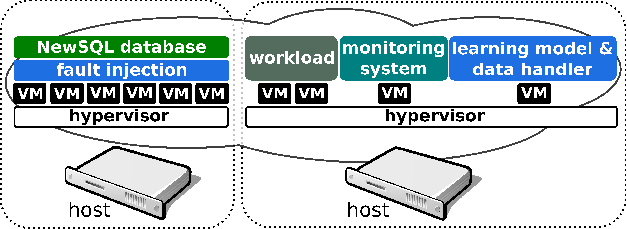
\includegraphics[width=1\textwidth]{inputs/img/experimental_scenario_extended_2}
  \caption{Experimental setup.}
  \label{fig:experimental_scenario_extended}
\end{figure}

\subsubsection{Components of Tejo and monitoring system.} As fault injection tools, we chose Dummynet (v3.0)~\cite{carbone2010dummynet} for network faults and \verb|stress-ng| (v0.01.30)~\footnote{stress-ng. \url{http://kernel.ubuntu.com/~cking/stress-ng/}} for disk, memory, and CPU faults. These tools provide a flexible, easy-to-reproduce way to inject arbitrary fault intensities. Table~\ref{tab:fault_campaign} lists the parameters of our fault injection campaign. The data handler component was implemented as a collection of python/shell scripts along with PostgreSQL database for datasets. We implemented our learning model using the Scikit-learn library~\cite{scikitlearn11}, from which we evaluated three learning algorithms: random forests~\cite{breiman2001random}, gradient boosting~\cite{friedman2006recent}, and SVM~\cite{svm_1995}. We used Ganglia as monitoring system. Our setup required additional Ganglia plug-ins for collecting performance counters of the workload and VoltDB. Every 15 seconds, we collected 147 performance metrics of each VM, and the average throughput and the 99$^{th}$ percentile latency from the served workload. 

			\begin{table*}[htdp]
				\begin{center}
\caption{The key parameters of Tejo for our fault injection campaign.}
  \label{tab:fault_campaign}
					\begin{tabular}{l c || r c c c }
						\multicolumn{2}{ l ||}{\bf Fault}&\multicolumn{3}{ c }{\bf Intensity ranges}&{\bf Unit} \\  
						&&Light&Medium&Heavy& \\  
						\hline
						\hline
						\multirow{3}{*}{\bf Network}&Pkt loss&1.6-3.2&4-5.6&6.4-8&\% \\
						&Latency&8-20&26-38&44-56&ms. \\
						&Limping&85-65&56-38&29-11&Mbps \\
						\hline
						\multicolumn{2}{ l ||}{\bf Memory}&73-79&82-88&91-97&\% \\
						\hline
						\multicolumn{2}{ l ||}{\bf Disk}&10-20&25-35&40-50&writers \\
						\hline
						\multicolumn{2}{ l ||}{\bf CPU}&19-39&49-69&79-99& \% \\
					\end{tabular}
				\end{center}
			\end{table*}



\subsubsection{NewSQL database and workloads.} We evaluated VoltDB (v4.x) as NewSQL database. We set the number of partitions VoltDB to 18 across a cluster of six VMs with failover mechanisms enabled. We varied the replication degree k from two to zero (i.e., replication disabled).  We evaluated VoltDB with two workloads, the popular TPC-C benchmark for OLTP~\footnote{TPC-C benchmark (v5.10). \url{http://www.tpc.org/tpcc/}},  and Voter~\footnote{Voter. \url{https://github.com/VoltDB/voltdb/tree/master/examples/voter.}}, a workload derived from leaderboard maintenance application for Japanese version of the ``American Idol''. We run Tejo for predicting anomalies in MongoDB cluster in our previous work~\cite{silvestre2014anomaly}.
